\chapter{Background}
\label{cha:background}
This chapter addresses the scientific background needed for this work. First, the general concept of digital signature systems and hash functions are elaborated. Afterwards, the most common concepts for post-quantum digital signature systems are explained. 

\section{Digital Signature Schemes}
% ! digital signature scheme -> assymetrisch (immer?) 
A \textit{digital signature scheme} uses a set of rules and a set of parameters to verify the identity of the originator and integrity of data.~\cite{cha:bg_digital_sign_schemes_NIST_standard1992} 

In this section, for explanatory reasons, data refers to a message being sent from one sender to a recipient across a network (e.g. LAN). The sender is the person signing the message, the recipient usually wants to verify the received message, therefore they are also referred to as signer and verifier. % 3. unabhängige Person auch als verifier?
The \textit{digital signature~$\sigma$} of a message, generated by a digital signature scheme, is a value dependent on some secret known only to the signer (usually the private key~$X$) and on the content of the message being signed. With the corresponding public key~$Y$ (without having access to the signer's private key $X$) the authenticity of the signature can be verified, either by the recipient directly or a third party: It is ensured that the message actually belongs to the signer - e.g. a lying signer trying to repudiate their signature, a fraudulent claimant arguing the message is theirs, or a message that has been tempered with can be detected.
% hier vlt Bild von Signatursystem?
% hier schutzziele erwähnen (vlt Liste?) -> recipient will bestätigung das nachricht wirklich vom empfänger, sender will dass recipient ihm keine falschen nachrichten unterschiebt
To ensure the above mentioned properties of digital signatures, a digital signature scheme consists of the following parts (see also Figure~\ref{img:digital_sign_system_simple}):~\cite{cha:bg_signature_schemes_book_menezes2018_1997} % gehört keygen wirklich zu signatursystem? -> ganze section beruht auf diesem Buch, wird das klar?

\begin{figure}
\centering
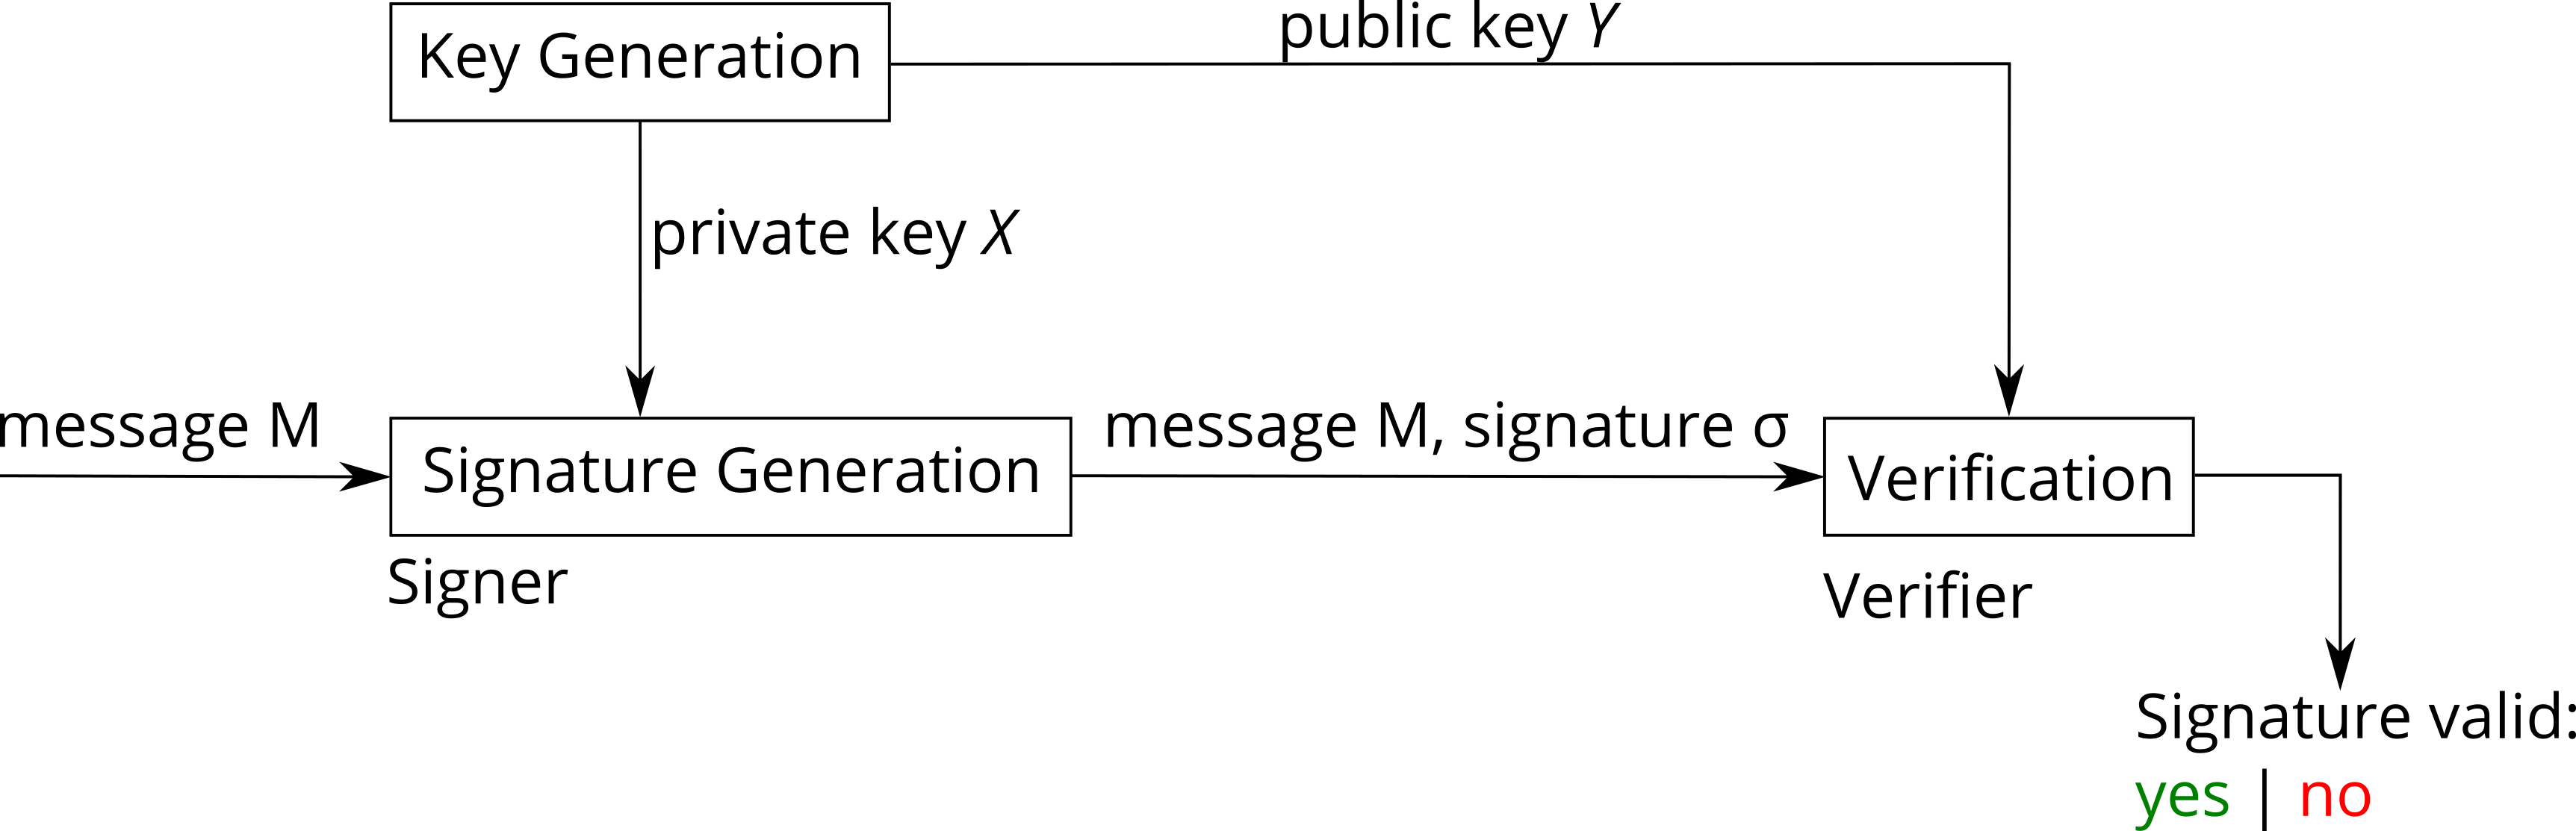
\includegraphics[width=\linewidth]{images/Background/Digital_Signaturesystem_Simple.png}
\caption{The general structure of a digital signature system. %Elke: Nur den ersten Satz als caption. Das hier nicht: The key generation algorithm creates the private key~$X$ and public key~$Y$, whereas $X$ is only known to the signer and $Y$ is made public for the verifier. The signer creates the message $M$ and signs it with the private key, using the signature generation algorithm. Afterwards, the so generated signature~$\sigma$ and the corresponding message~$M$ are sent to the verifier. The verifier checks the validity of the message and the corresponding signature with the public key (that is already known after key generation and distribution) and the verification algorithm. If the verification algorithm evaluates returns a valid result, the verifier can trust the message or otherwise knows it has been tempered with).
}
\label{img:digital_sign_sytem_simple}
\end{figure} 

\begin{enumerate}
\item The \textit{key generation algorithm} creates a private key~$X$ used for signature generation, and a public key $Y$ used by the recipient for signature verification. Both keys are mathematically dependent from each other, in which way is determined by the specific type of signature scheme (e.g. the Winternitz signature scheme, see Section~\ref{sec:WOTS_keygen}). % und auch noch von weiteren Leuten die Originalität von Nachricht prüfen wollen? Aber in meinem runtergebrochenen Beispiel nur 2 Leute, außerdem wird nicht erklärt dass auch key signiert wird
\item The \textit{signature generation algorithm} creates the digital signature~$\sigma$ of a message with the private key $X$ of the signer and the content of the message.
\item The \textit{verification algorithm} is used by the recipient or a third party to verify the authenticity of the signature~$\sigma$ and the corresponding message with the public key $Y$.
\end{enumerate}
% Y muss vor signieren der Nachricht veröffentlich werden

% Bild / Schema einfügen

% es wird message digest signiert
% Überleitung zu Hashfunctions

\section{Definition of Hash Functions} 
The security of \textit{One-Time Signature Schemes} (see section~\ref{sec:one-time_sign_schemes}) %Elke: Man könnte auch sagen, dass Signaturverfahren i. Allg. Hashfunktionen verwenden ...
 is based on cryptographic secure hash functions. A hash function is a function that can be computed efficiently and maps strings of arbitrary length to strings of fixed length~\cite{cha:bg_hashfunctions_thesis_matusiewicz2007}. Therefore a hash function $h$ is defined as any function $h: X \rightarrow Y$, with $|X| = X_{len}$ (arbitrary length) and $|Y| = Y_{len}$ (fixed length)~\cite{cha:bg_hashfunctoins_Stinson2006}. A hash function is considered \textit{cryptographically secure} if it has the following  properties:~\cite{cha:bg_hashfunctions_BASIC_DEFINITIONS_Springer2004} 

% M ist auch die ungehashte message später -> dort umbenennen zB M_sent \\ hashfunction hat fixe outputlänge? also M fix?
\begin{enumerate} % fotos einfügen?
	\item \textbf{Preimage-Resistance / One-wayness}
	 A hash function $h$ is preimage-resistant if given the output value of the function, it is computationally infeasible to find any input which generates this output, i.e. finding any preimage $x$ such that $h(x) = y $ when given any $y$. 

\begin{minipage}[t]{.5\linewidth}
          	\raggedright
            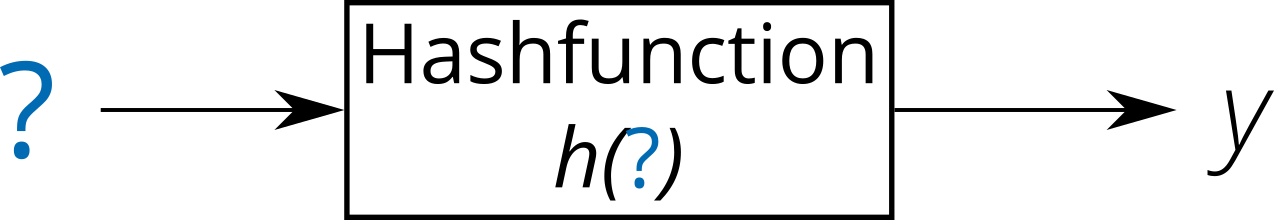
\includegraphics[width=.8\linewidth]{images/Background/preimage_res_horizontal.png}
	      \end{minipage} 

	\item \textbf{Second Preimage-Resistance}
	A hash function $h$ is second preimage-resistant, if given any input value and the corresponding output, it is computationally infeasible to find another distinct
input that produces the same output, i.e. given any $x$ finding a second preimage $x \neq x'$ such that $h(x) = h(x')$. % oder erst formel -> dann beschreibung dran?

\begin{minipage}[t]{.6\linewidth}
          	\raggedright
            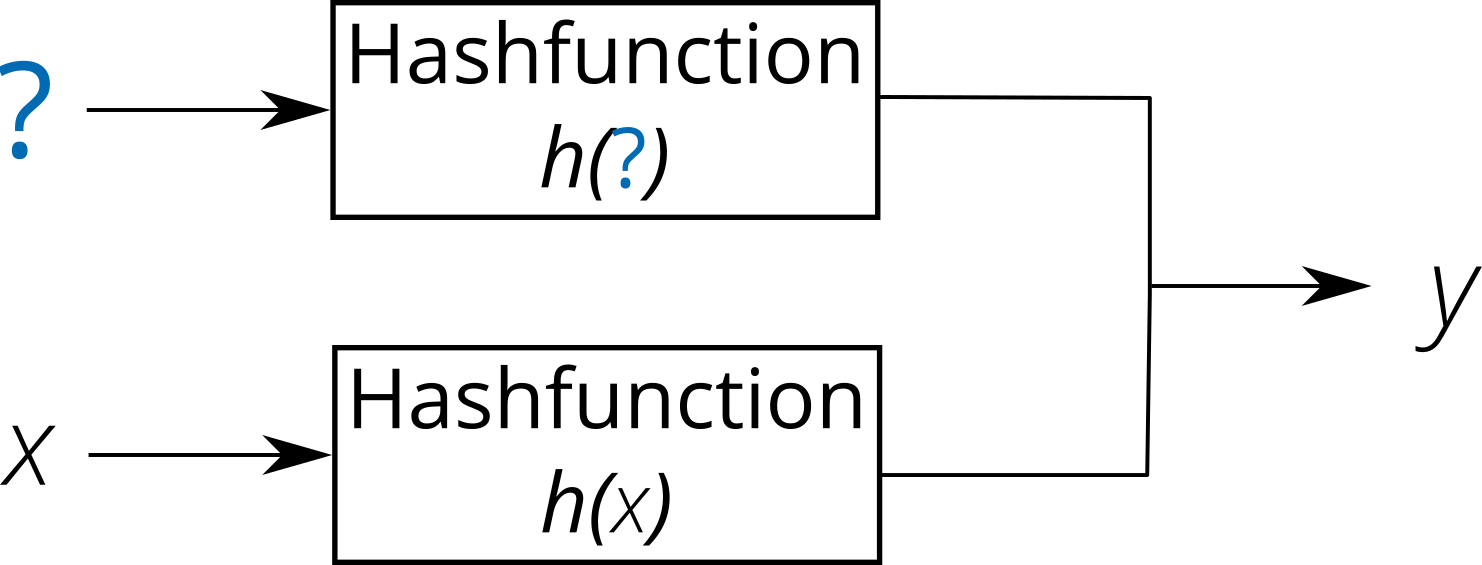
\includegraphics[width=.8\linewidth]{images/Background/second_preimage_res_horizontal.png}
	      \end{minipage} 
	
	\item \textbf{Collision Resistance}
	A hash function $h$ is called collision-resistant, if it is computationally infeasible to find a pair of different inputs $x, x'$ that map to the same output value, such that $h(x) = h(x')$.


\begin{minipage}[t]{.6\linewidth}
          	\raggedright
            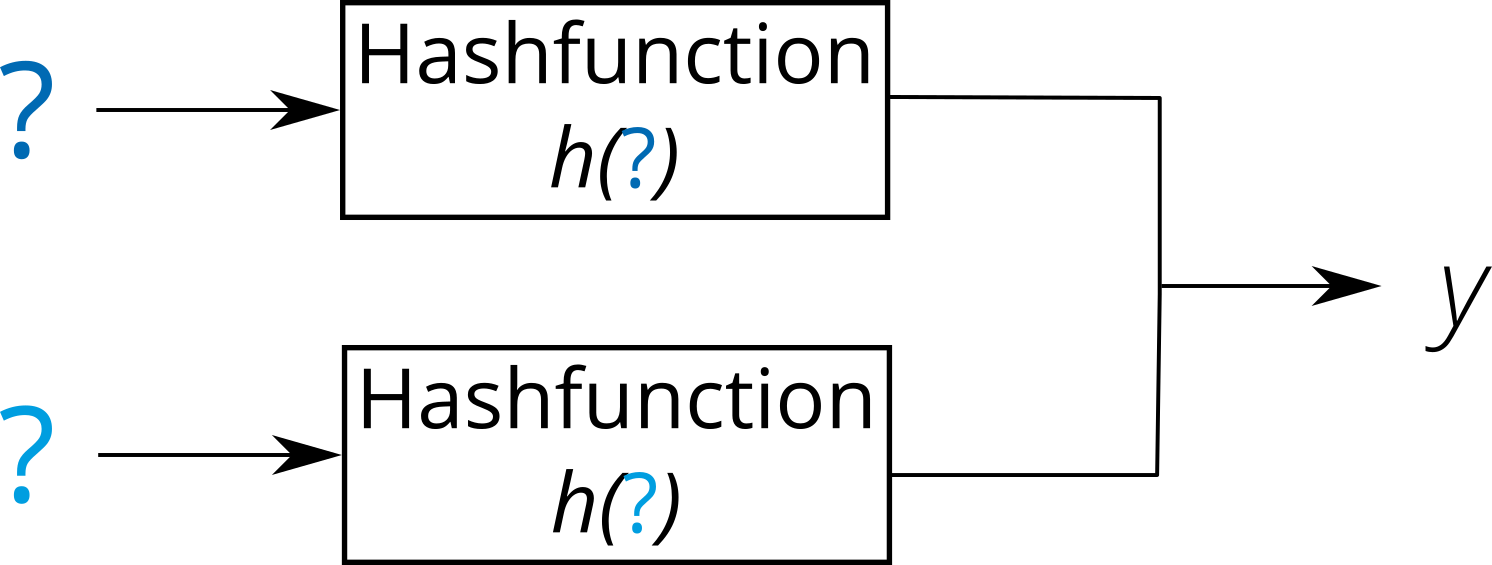
\includegraphics[width=.8\linewidth]{images/Background/collission_res_horizontal.png}
	      \end{minipage}
	      
\end{enumerate}	      


\section{One-Time Signature Schemes}
\label{sec:one-time_sign_schemes}
This section is based on the work of Buchmann et al~\cite{book_pqc_bernstein_2004}. 
% ONE-Time Signature scheme anmerken / erklären
The two signature schemes Lamport-Diffe and Winternitz are both \textit{one-time signature schemes (OTS)}, meaning the public and private key can be used \textbf{once}, for signing a single message. If they are used for generating more than one signature, the signature can be forged. % vlt rauslöschen einfach
The following types of functions are used for the Lamport-Diffie One-Time Signature Scheme and the Winternitz One-Time Signature Scheme: 
The cryptographic hash function~$h$ is preimage resistant, second preimage-resistant and collision resistant, it is applied to the original message and generates the message digest.
The one-way function~$f$ is a hash function that is at least preimage-resistant and takes a fixed input length, because it is applied to the message digest.% später wird Benutzung von h und f noch sichtbar
% hier erklären was one time signature scheme ist & dass LD-OTS und Winternitz-OTS erklärt werden

\begin{equation}
\label{eq:basic_hashfunc}
\textbf{Cryptographic hash function h: } \lbrace 0,1 \rbrace^* \rightarrow \lbrace 0,1 \rbrace^n
\end{equation}

\begin{equation}
\label{eq:one-way-func}
\textbf{One-way function f: } \lbrace 0,1 \rbrace^n \rightarrow \lbrace 0,1 \rbrace ^n
\end{equation}


\subsection{Lamport-Diffie One-Time Signature Scheme (LD-OTS)}
The Lamport–Diffie one-time signature scheme (LD-OTS) was first proposed by Leslie Lamport in 1979~\cite{lamport_signature_scheme_1979}. 

\subsubsection{LD-OTS Key Generation}
The private key X consists of $2n$ bit strings, each of length $n$, chosen at random. % n ist security parameter

\begin{equation}
\label{eq:ldots_sign_key}
X = \left(x_{0}\left[0\right], x_{0}\left[1\right], x_{1}\left[0\right], x_{1}\left[1\right], \cdots, x_{n-1}\left[0\right], x_{n-1}\left[1\right] \right)
\end{equation}
The public key $Y$ is created out of the private key $X$. For each $x_i[j] \in X, 0 \leq i \leq n-1, j \in \lbrace 0,1 \rbrace$, the one-way function~f (see Equation~\ref{eq:one-way-func}) is applied.

\begin{equation}
y_i[j] \in Y = f(x_i[j]), 0 \leq i \leq n-1, j \in \lbrace 0,1 \rbrace
\end{equation}

\begin{equation}
Y = \left( 
y_{0}\left[0\right], y_{0}\left[1 \right], y_{1}\left[0\right], y_{1}\left[1\right], \cdots, y_{n-1}\left[0\right], y_{n-1}\left[1\right]
\right)
\end{equation}

\subsubsection{LD-OTS Signature Generation} % m has fixed length
Before signing, the public key $Y$ has to be published.
The private key $X$ (see Equation~\ref{eq:ldots_sign_key}) is used to sign the message $M \in \lbrace 0,1 \rbrace^*$. 
The cryptographic hash function $h$ (see Equation~\ref{eq:basic_hashfunc}) is applied to $M$ in order to get the hash digest $m$ of fixed length $n$.

\begin{equation}
\label{eq:hash_message}
m = h(M) = (h_{0}, \cdots, h_{n-1})
\end{equation} % Elemente von m ENTWEDER m_i ODER h_i
For each $h_i \in m$, the corresponding $x_i[h_i]$ out of private key $X$ is chosen, resulting in signature $\sigma$ for message $m$.
% h_i in m_i umbenennen oder umgekehrt -> konsequent bleiben
\begin{equation}
\sigma = \left(
x_0 \left[ h_0 \right], x_1\left[ h_1 \right], \cdots, x_{n-1}\left[ h_{n-1}\right]
\right) = (\sigma_0, \cdots, \sigma_{n-1})
\end{equation}

\subsubsection{LD-OTS Verification}
After receiving a message $M$ with the corresponding signature $\sigma$, the verifier calculates the message digest $h(M) = m$. 
To verify the given signature $\sigma$, it is necessary to check the following condition.
\begin{equation}
\left(
f(\sigma_0), \cdots, f(\sigma_{n-1})
\right) =
\left(
y_0[h_0], \cdots, y_{n-1}[h_{n-1}]
\right)
\end{equation}
If the condition is true, the signature is valid.

% nochmal extra auf Einmalverwendung hinweisen
% table with properties i.e.
% keygen+sign+verify time / aufwand / speicherverbrauch -> Positiv: schnelle signatur+keygen Negativ: Viel Speicherverbrauch
% Überleitung zu Winternitz weil diese Vorteil kürzerer Signatur aufweisen

\subsection{Winternitz One-Time Signature Scheme (W-OTS)}
LD-OTS signatures are efficient to calculate but have a huge size and therefore need a lot of memory. The Winternitz one-time signature scheme (W-OTS) generates signatures with substantially shorter size. W-OTS uses the same hash function (Equation~\ref{eq:basic_hashfunc}) and one-way function (Equation~\ref{eq:one-way-func}) as LD-OTS. %genauer beschreiben evtl

\subsubsection{W-OTS Key Generation}
\label{sec:WOTS_keygen}
First, two parameters are selected: The Winternitz-Parameter $w \geq 2$ and the security parameter $n$. When increasing $w$, the signature size will decrease linearly and the effort for key generation, signing and verification will increase exponentially. As $n$ is the length of the message digest, increasing it leads to higher security because it increases the collision resistance of the hash function. % weil mehr Winternitz-Ketten generiert werden, je kleiner w ist, reduziert ein hohes w die Signaturgröße
% The Winternitz parameter w enables space/time trade-offs.

% bezieht sich auf #stücke in die m geteilt wird
\begin{equation}
\label{eq:t1}
t_1 = \ceil[\Bigg]{\frac{n}{w}}
\end{equation}

% bezieht sich auf #stücke in die checksum geteilt wird
\begin{equation}
\label{eq:t2}
t_2 = \ceil*{\frac{\floor*{\log_2 t_1} + 1 + w}{w} }
\end{equation}

% anzahl stücke von signatur M || C am ende
\begin{equation}
\label{eq:t}
t = t_1 + t_2
\end{equation}
The private key $X$ consists of $t$ bit strings, each of length $n$ chosen at random.

\begin{equation}
\label{eq:wots_privkey}
X = (x_0, \cdots, x_{t-1})
\end{equation}
The public key $Y$ is generated by applying the one-way function~$f$ to each element $x_i  \in X$  consecutively $2^w - 1$ times. % hier sieht man dass höheres w -> höherer Aufwand Keygen

\begin{equation}
y_i \in Y =  f^{2^w-1}(x_i), 0 \leq i \leq t-1 
\end{equation}

\begin{equation}
Y = (y_0, \cdots, y_{t-1})
\end{equation}
Each $y_i \in Y$ is a bit string of length $n$. The public key $Y$ has to be published before the signature can be generated.

\subsubsection{W-OTS Signature Generation}
For signing a message $M \in \lbrace 0,1 \rbrace^*$, the cryptographic hash function~h (see Equation~\ref{eq:basic_hashfunc}) is applied to $M$ (see Equation~\ref{eq:hash_message}). The resulting hash digest $m$ is split into $t_1$ bitstrings of length $w$. If $m$ is not divisible by $w$, it is necessary to add leading zeros to $m$ before splitting.

\begin{equation}
\label{eq:hash_digest_split}
m = m_0 \concat m_1 \concat \cdots \concat m_{t_1-1}
\end{equation}
Each bitstring $m_i \in m$ is converted to its decimal representation in order to calculate the checksum $c$.
% checksum t2 Teile der Länge w teilbar

\begin{equation}
\label{eq:checksum_calculation}
c = \sum_{i = 0}^{t_{1}-1}(2^w-m_i)
\end{equation}
The checksum $c$ is divided into $t_2$ bitstrings of length $w$. In order to divide $c$ this way, it can be necessary to add leading zeros to $c$ as a padding.
\begin{equation}
c = c_0 \concat c_1 \concat \cdots \concat c_{t_2 - 1}
\end{equation}
Afterwards, $m$ and $c$ are concatenated to one block~$B$. This leads to $t$ bitstrings of length $w$ in total, as $t = t_1 + t_2$.

\begin{align}
\label{eq:block_B_out_of_M_and_C}
B &= m \concat c  \\ 
&= m_0 \concat \cdots \concat m_{t_1 - 1} \concat c_0 \concat \cdots \concat c_{t_2 - 1} \nonumber \\
&= b_0 \concat \cdots \concat b_{t-1} \nonumber
\end{align}
The signature $\sigma$ is calculated by applying the one-way function~$f$ to each part of the private key $X$ (see Equation~\ref{eq:wots_privkey}) several times: The element $b_i \in B$ determines the amount of times the hash function $f$ is applied to the corresponding $x_i \in X$.

\begin{equation}
\sigma = (f^{b_0}(x_0), f^{b_1}(x_1), \cdots, f^{b_{t-1}}(x_{t-1})) = (\sigma_0, \cdots, \sigma_{t-1})
\end{equation}

\subsubsection{W-OTS Verification}
Given a signature $\sigma$ and message $M$, the hash digest $m$ is generated (see Equation~\ref{eq:hash_message}). Afterwards, the block $B$ is generated out of~$m$ as shown in the previous section (see Equations~\ref{eq:hash_digest_split} to~\ref{eq:block_B_out_of_M_and_C}). To check if the given signature is valid, the one-way function~$f$ is applied $2^w - 1 - b_i$ times to each $\sigma_i \in \sigma$. The result is compared to the corresponding $y_i \in Y$.

\begin{equation}
(f^{(2^w-1)-b_0}(\sigma_0), \cdots, f^{(2^w - 1) - b_{t-1}}(\sigma_{t-1})) \? (y_0, \cdots, y_{t-1})
\end{equation}
If each $f^{2^w-1-b_i}(\sigma_i) = y_i$, the signature is valid because $\sigma_i = f^{b_i}(x_i)$ and therefore

\begin{gather}
f^{2^w-1-b_i}(\sigma_i) = f^{2^w-1}(x_i) = y_i \\
0 \leq i \leq t-1 \nonumber
\end{gather}

\subsubsection{W-OTS Example Calculation}
This section contains an example calculation of W-OTS, including key generation, signature generation, and signature verification.

\begin{enumerate}

\item The first step is choosing the following parameters:
$n=3, w=2, \text{message digest } m = 101, {\text{one-way function } f:\{0,1\}^{3} \rightarrow \{0,1\}^{3}, x \rightarrow x+2 \text{ mod } 8}$

% ceilings of t_2 are a bit ugly. Maybe fix later
\item Calculating $t_1, t_2, t$: \\
$t_1 = \ceil{\frac{n}{w}} = \ceil{\frac{3}{2}} = 2, t_2 = \ceil*{\frac{\floor*{\log_2 t_1} + 1 + w}{w} } = \ceil*{\frac{\floor*{\log_2 2} + 1 + 2}{2} } = 2, {t = t_1 + t_2 = 2+2 = 4}$

\item Choosing the private key $X$ with $t=4$ random bit strings of length $n=3$: \\
$X = (x_0, \cdots, x_{t-1}) = (x_0, x_1, x_2, x_3) = 
\begin{psmallmatrix}
1 & 1 & 0 & 1\\
0 & 1 & 1 & 1\\
1 & 1 & 1 & 0
\end{psmallmatrix} \in \{0,1\}^{(3,4)} $

\item Calculating the public key $Y$ from $X$ by applying $f$ to each element in $X$ for $2^{w-1} = 2$ times:	
$Y = (y_0, \cdots, y_{t-1}) = (y_0, y_1, y_2, y_3) = 
\begin{psmallmatrix}
0 & 0 & 1 & 0 \\
0 & 1 & 1 & 1 \\
1 & 1 & 1 & 0
\end{psmallmatrix} \in \{0,1\}^{(3,4)} $ 

\item To make $m$ divisible by $w$, a leading zero is inserted. Then it is split in blocks of length $w$: $m = 01 \concat 01 = m_0 \concat m_1$. These blocks are used for the checksum calculation: \\ $c = (2^w - m_0) + (2^w - m_1) = (4-1)+(4-1)=6$. To make $c$ divisible by $w$ as well, one leading zero is added to the binary representation of $c$. Then, splitting $c$ in blocks of length $w$ yields $c = 01 \concat 10 = c_0 \concat c_1$.

\item The block $B$ is generated by concatenating $m$ and $c$: \\ $B = m_0 \concat m_1 \concat c_0 \concat c_1 = b_0 \concat b_1 \concat b_2 \concat b_3 = 01 \concat 01 \concat 01 \concat 10 $.

\item %The signature $\sigma$ is created by applying $f$ to each element in $X$.
%The block $B$ determines the amount of applying $f$ to $X$
The signature $\sigma$ of $m$ is determined by the parameter $B$ and one-way function $f$: \\ % hier besser erklären dass man dezimalrepr. von B und X nimmt?
$\sigma = (f^{b_0}(x_0), f^{b_1}(x_1),f^{b_2}(x_2),f^{b_3}(x_3)) = (f^1(5),f^1(7),f^1(3),f^2(6)) = (\sigma_0, \sigma_1, \sigma_2, \sigma_3) = 
\begin{psmallmatrix}
1 & 0 & 1 & 0 \\
1 & 0 & 0 & 1 \\
1 & 1 & 1 & 0
\end{psmallmatrix} \in \{0,1\}^{(3,4)} $

\item The verifier knows $Y, w, n$ and therefore $t_1, t_2$ and $t$. After receiving $m, \sigma$ from the signer, the block $B$ is calculated as well as explained in the previous steps. The validity of the signature $\sigma$ is checked by calculating: \\
$( f^{2^w-1-b_0}(\sigma_0), f^{2^w-1-b_1}(\sigma_1), f^{2^w-1-b_2}(\sigma_2), f^{2^w-1-b_3}(\sigma_3)) = (f^2(7) , f^2(1), f^2(5), f^1(2)) = \begin{psmallmatrix}
0 & 1 & 0 & 1 \\
1 & 0 & 0 & 0 \\
1 & 1 & 1 & 0
\end{psmallmatrix} \in \{0,1\}^{(3,4)} $
Because these values are the same as in the public key $Y$, $\sigma$ is valid. 

\end{enumerate}

% dann überleiten -> merkle trees, diese benutzen um OTS zu "Mehrmaligen" Signatursystemen zu machen 

\section{Merkle Signature Scheme (MSS)} 
%!! Zitierung fehlt von Buchmann
The main disadvantage of the one-time signature schemes introduced in Section~\ref{sec:one-time_sign_schemes} is the restriction to use each key pair (consisting of private key~$X$ and public key~$Y$) for only one signature. This is inadequate for most practical situations, because the key generation as well as the key distribution take a lot of time and effort that could be saved otherwise.
To solve this problem, Merkle~\cite{cha:bg_merkletrees_Merkle_1979} proposed the concept of using a binary hash tree, where each leaf represents a different one-time key pair. The root of the tree is the public key $Y_{MSS}$  which combines the one-time key pairs at the leafs. With a tree depth $d$, $2^d$ one-time key pairs and corresponding signatures can be generated. % achtung: bei RSA mehr, possibly unendlich
This concept is denoted as \textit{Merkle signature scheme (MSS)} and it works with any cryptographic hash function and any one-time signature scheme. 
% -> maybe better: works with any scheme but W-OTS "works best"?
In the following sections, the cryptographic hash function~$h$ (see Equation~\ref{eq:basic_hashfunc}) is used. 
% besser einbinden :D
%The idea is to use a complete binary hash tree to reduce the validity of an arbitrary but fixed number of one time verification keys to the validity of one single public key, the root of the hash tree. 

\subsection{MSS Key Generation}
For a depiction of the Merkle tree referenced in this section, see Figure~\ref{img:merkle_tree}.
The signer chooses the tree depth~$d$ where $d \geq 2$, and generates $2^d$ one-time key pairs $(X_j, Y_j)$ where $0 \leq j \leq 2^d-1$, with $X_j$ being the private key and $Y_j$ the corresponding public key. The \textit{leaves} of the Merkle tree are the hash digests $H_{i,j}$ of the public key $Y_j$.
\begin{gather}
\label{eq:leaf_merkle_tree:hash_digest_publ_key_Y}
H_{i,j} = h(Y_j) \\
i = d \nonumber \\  
0 \leq j \leq 2^d - 1 \nonumber
\end{gather}
The \textit{inner nodes} of the Merkle tree are computed as follows: Each parent node $H_{i,j}$ is the hash digest of the concatenation of its direct two children: % $H_{i+1,j}$ and $H_{i+1,j+1}$.

% ! wichtig dass 0 <= i < d weil Blätter zählen nicht mit
\begin{gather}
H_{i,j} = h(H_{i-1,2j} \concat H_{i-1,2j+1}) \\
1 \leq i \leq d \nonumber \\ 
0 \leq j < 2^{d - i} \nonumber
\end{gather} 
The \textit{root} of the Merkle tree is the MSS public key~$Y_{MSS}$. The MSS private key~$X_{MSS}$ is the collection of one-time signature keys generated before constructing the Merkle tree.
% Y_mss = H_d,0 because d=height of tree
\begin{align}
X_{MSS} &= (X_0, \cdots, X_j, \cdots, X_{2^d - 1} ) \\
Y_{MSS} &= H_{d,0} \nonumber
\end{align}


\begin{figure}
\label{img:merkle_tree}
\centering
% unsichtbare Kante: edge from parent[draw=none]
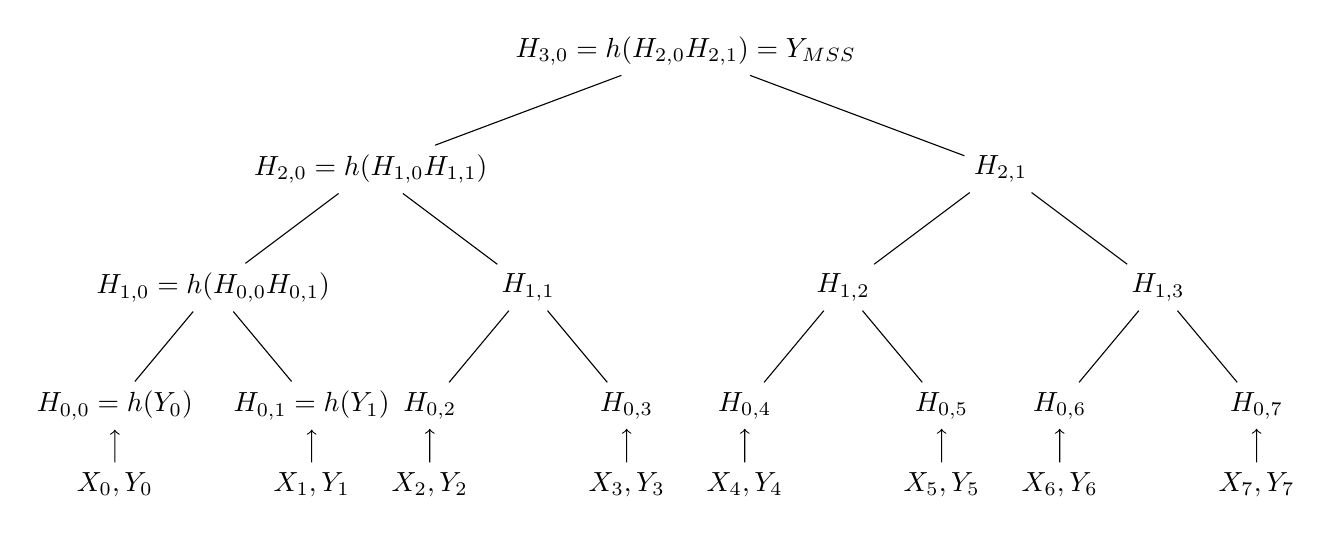
\begin{tikzpicture} 
[
    level 1/.style = {sibling distance = 8cm},
    level 2/.style = {sibling distance = 4cm},
    level 3/.style = {sibling distance = 2.5cm},
    level 4/.style = {level distance = 1cm}
]
\node {$H_{3,0} = h(H_{2,0} \concat H_{2,1}) = Y_{MSS}$}
	child { node {$H_{2,0} = h(H_{1,0} \concat H_{1,1})$} 
		child { node {$H_{1,0} = h(H_{0,0} \concat H_{0,1})$}
			child{ node {$H_{0,0} = h(Y_0)$}
				child{ node {$X_0, Y_0$} edge from parent[<-]
				}	
			}
			child{ node {$H_{0,1} = h(Y_1)$}
				child{ node {$X_1, Y_1$} edge from parent[<-]
				}			
			}		
		} 
		child { node {$H_{1,1}$}
			child{ node {$H_{0,2}$}
				child{ node {$X_2, Y_2$} edge from parent[<-]
				}			
			}
			child{ node {$H_{0,3}$}
				child{ node {$X_3,Y_3$} edge from parent[<-]
				}			
			}		
		}	
	}
	child { node {$H_{2,1}$} 
		child { node {$H_{1,2}$}
			child {node {$H_{0,4}$}
				child{ node {$X_4, Y_4$} edge from parent[<-]
				}			
			}
			child {node {$H_{0,5}$}
				child{ node {$X_5,Y_5$} edge from parent[<-]
				}			
			}		
		}
		child { node {$H_{1,3}$}
			child {node {$H_{0,6}$}
				child{ node {$X_6,Y_6$} edge from parent[<-]
				}			
			}
			child {node {$H_{0,7}$}
				child{ node {$X_7,Y_7$} edge from parent[<-]
				}			
			}
		}	
	}
	;
\end{tikzpicture} % klarmachen dass h1,1 = hash(h2,1|h2,2) usw
\caption{Merkle tree of depth $d=3$. The composition of the tree is depicted in detail on the left branch, each node consists of the hash digest of its concatenated children. The leafs are the hash digest of their corresponding public key (see Equation~\ref{eq:leaf_merkle_tree:hash_digest_publ_key_Y}).}
\end{figure}
% soll treehash algo hier auch erklärt werden?

\subsection{MSS Signature Generation}
For a depiction of the Merkle tree referenced in this section, see Figure~\ref{img:merkle_tree_signature_gen}.
%The one-time key pairs are used successively for generating signatures.  
To sign a message $M$, the signer calculates the hash digest $m = h(M)$ of length $n$ (see Equation~\ref{eq:hash_message}). Then, by using a chosen one-time signature scheme, the one-time signature $\sigma_{s/OTS}$ of $m$ is generated with a one-time key $X_s, s \in \{0, \cdots, 2^d - 1\}, X_s \in X_{MSS}$. 

\begin{equation}
\label{eq:merkle_s/OTS_signature}
\sigma_{s/OTS} \leftarrow_{sign} (X_s, m) 
\end{equation}
% das folgende ist vom Konzept her falsch? (Vor allem folgende 2 Sätze) -> steht so in Lehrbuch
\textcolor{red}{The corresponding $Y_s$ is also part of the signature}.% <- "nicht wirklich" -> LD-OTS, WOTS anschauen was da mitgegeben wird jeweils in Signatur
The verifier checks the authenticity of the signature by calculating a part of the Merkle-Tree, see Figure~\ref{img:merkle_tree_signature_gen}. Therefore, additional information about the Merkle tree is included into the signature: The index $s$ and an authentication path for the verification key $Y_s$. The authentication path $A_s$ consists of a sequence of nodes $a_i$ in the Merkle tree:

% a_{d-1}, NOT a_{d} because this would be the root
% a_i vlt rausnehmen aus Sequenz?
\begin{equation}
A_s = (a_0,\cdots, a_i, \cdots, a_{d-1})
\end{equation}
Each node $a_i \in A_s$ is calculated as follows:
% !! floor probably also necessary for first equations
\begin{align}
\label{eq:auth_path_calculation_merkle_tree}
&a_{i} = H_{i, j} \\
&j = 
\left\{\begin{matrix} \nonumber
\floor{s/2^i}-1 \text{ if } \floor{s/2^i} \equiv 1 \mod{2} \\
\floor{s/2^i}+1 \text{ if } \floor{s/2^i} \equiv 0 \mod{2}
\end{matrix}\right.  \nonumber \\
&0 \leq i \leq d-1 \nonumber
\end{align}
Because of the index $s$, the verifier knows the leaf-position of $Y_s$. In combination with the authentication path $A_s$, the verifier can construct a path from the leaf $h(Y_s)$ to the root of the Merkle tree, see Figure~\ref{img:merkle_tree_signature_gen}. % explain more detailed that root is made public BEFORE one-time key Y/the signature is made public


% ? path h2,0 - h1,0 and h1,1 - h0,0 also with arrows?
% in caption: "path from leaf to the root" not entirely correct, cyan nodes also part of the path?
\begin{figure}
\label{img:merkle_tree_signature_gen}
\centering
% unsichtbare Kante: edge from parent[draw=none]
\begin{tikzpicture} 
[
    level 1/.style = {sibling distance = 8cm},
    level 2/.style = {sibling distance = 4cm},
    level 3/.style = {sibling distance = 2.5cm},
    level 4/.style = {level distance = 1cm}
]
\node [darkblue_tud] {$H_{3,0} = p_3 \? Y_{MSS}$ }
	child { node [darkblue_tud] {$H_{2,0} = p_2$ } edge from parent[<-]
		child { node [cyan_tud] {$H_{1,0} = a_1$} edge from parent[-, black]
			child{ node {$H_{0,0} = h(Y_0)$}
				child{ node {$X_0, Y_0$} edge from parent[<-]
				}	
			}
			child{ node {$H_{0,1}$}
				child{ node {$X_1, Y_1$} edge from parent[<-]
				}			
			}		
		} 
		child { node [darkblue_tud] {$H_{1,1} = p_1$}  edge from parent[<-]
			child{ node [cyan_tud]{$H_{0,2} = a_0$} edge from parent[-, black]
				child{ node {$X_2, Y_2$} edge from parent[<-]
				}			
			}
			child{ node [darkblue_tud] {$H_{0,3} = p_0$} edge from parent[<-]
				child{ node {$X_3, \textcolor{cyan_tud}{Y_3}$} edge from parent[<-]
				}			
			}		
		}	
	}
	child { node [cyan_tud] {$H_{2,1} = a_2$} 
		child { node {$H_{1,2}$}
			child {node {$H_{0,4}$}
				child{ node {$X_4, Y_4$} edge from parent[<-]
				}			
			}
			child {node {$H_{0,5}$}
				child{ node {$X_5,Y_5$} edge from parent[<-]
				}			
			}		
		}
		child { node {$H_{1,3}$}
			child {node {$H_{0,6}$}
				child{ node {$X_6,Y_6$} edge from parent[<-]
				}			
			}
			child {node {$H_{0,7}$}
				child{ node {$X_7,Y_7$} edge from parent[<-]
				}			
			}
		}	
	}
	;
\end{tikzpicture}
\caption{Merkle signature generation and verification for $d=3, s=3$. The nodes $H_{0,2}, H_{1,0}, H_{2,1}$ are in the \textcolor{cyan_tud}{authentication path $A_3 = (a_0, a_1, a_2)$} calculated by the signer, \textcolor{cyan_tud}{$Y_3$} is the corresponding \textcolor{cyan_tud}{one-time public key}. The \textcolor{darkblue_tud}{path $P_s = (p_0, p_1, p_2, p_3)$} is calculated by the verifier, also indicated by the arrows. If the root $p_3$ calculated by the verifier matches the public key $Y_{MSS}$, \textcolor{red}{the one-time public key $Y_3$ is valid}.}
\end{figure}
In summary, one MSS signature contains the following elements:
% Ys not part of sigma_s?
\begin{equation}
\label{eq:complete_merkle_signature_for_one_Ys}
\sigma_s = (\textcolor{red}{Y_s}, s,\sigma_{s/OTS}, A_s) 
\end{equation}

\subsection{MSS Signature Verification}
For a explanatory depiction of the Merkle tree referenced in this section, see Figure~\ref{img:merkle_tree_signature_gen}.
After receiving the Merkle signature $\sigma_s$, \textcolor{red}{the verifier uses the one-time public key $Y_s$ to verify} % -> wrong, needs to be changed
 the one-time signature $\sigma_{s/OTS}$ of message digest $m$ (see also Equation~\ref{eq:merkle_s/OTS_signature}) with the signature verification algorithm of the corresponding one-time signature scheme.
%\begin{equation}
%(\sigma_{s/OTS},m) \rightarrow{verify} 
%\end{equation}
Afterwards, the verifier has to check the authenticity of $Y_s$ itself by creating the path $P_s$ from $Y_s$ to the root of the Merkle tree:

\begin{equation}
P_s = (p_0, \cdots, p_d)
\end{equation}
The path $P_s$ is constructed by using the index $s$ and the authentication path $A_s$ (see Figure~\ref{img:merkle_tree_signature_gen}):

\begin{align}
\label{eq:merkle_verifier_path_calculation}
&p_0 = h(Y_s) \\
&p_{i} = 
\left\{\begin{matrix} \nonumber
h(a_{i-1} \concat p_{i-1}) \text{ if } \floor{s/2^{i-1}} \equiv 1 \mod{2} \\
h(p_{i-1} \concat a_{i-1}) \text{ if } \floor{s/2^{i-1}} \equiv 0 \mod{2}
\end{matrix}\right.  \nonumber \\
&0 \leq i \leq d  \nonumber 
\end{align}
The authentication of the one-time verification key $Y_s$ is only successful if the root $p_d$ calculated by the verifier matches the public key $Y_{MSS}$.

\section{Leighton-Micali Signature Scheme (LMS)}

\subsection{LMS Key Generation}

\subsection{LMS Signature Generation}

\subsection{LMS Signature Verification}


\section{Extended Merkle Signature Scheme (XMSS)}

\subsection{XMSS Key Generation}

\subsection{XMSS Signature Generation}

\subsection{XMSS Signature Verification}


% ganz am Ende: Übersichtstabelle zu allen Zeit/Speicheraufwandszeiten
% MSS key pair generation requires the computation of 2^d one-time key pairs and 2^(d+1)-1 evaluations of the hash function.
% WOTS keygen+sign+verify time / aufwand / speicherverbrauch -> Positiv: Wenig Speicherverbrauch, kleinere Signatur als bei Lamport-Diffie!

% Facts Merkle-Tree:
% - Each public key (== root of the tree) can only be used to sign fixed number of messages - typically 2^n (weil 2^d = #Blätter von Baum mit Höhe d)
% + public key: short, only one hash value
% - signature size: huge, contains d public keys (für jede Höhe des Baumes eine, ein a_i + die one-time signatur an sich)
% - Berechnung public key (root): berechnen + speichern von 2^n ots-keys -> vlt kürzer mit treehash algo
% -> tradeoff zw. speicher+zeit: private keys S_i, deterministisch von kurzem secret seed S. Wenig Speicher für seed benötigt, dafür Zeit für Berechnung von secret keys->signature generation benötigt

% \subsection{XMSS}
% xmss kurz beschreiben: WOTS+merkle trees = xmss
% - hypertress
% - nur 1 seed gespeichert, aus dem Zufall erzeugt wird, aus dem private keys erzeugt werden (herausstellen, was unterschied zu merkle trees ist)	